\chapter{Aplicația web Next.js}

\section{Structura proiectului}
Aplicația de frontend este construită cu Next.js 16 și React 19 (vezi \texttt{package.json}). Folosește \textit{App Router}-ul Next.js, ceea ce înseamnă că rutele sunt definite implicit prin structura folderelor din directorul \texttt{app/}. Două rute sunt publice și separate de zona autentificată:
\begin{itemize}
    \item \texttt{app/login/} — formular de autentificare;
    \item \texttt{app/register/} — formular de înregistrare;
    \item \texttt{app/setup/} — \textit{setup wizard}-ul afișat când backend-ul răspunde cu \texttt{is\_fresh: true}.
\end{itemize}

Restul aplicației trăiește sub \texttt{/dashboard/...} și folosește un layout comun definit în \texttt{layout.tsx}. Acesta verifică, la fiecare reîncărcare, profilul curent prin \texttt{fetchProfile()} și redirecționează către \texttt{/login} dacă răspunsul este \texttt{401}. Tot el inserează \texttt{SidebarProvider}-ul, breadcrumb-urile dinamice și butonul de schimbare a temei (light/dark).

Sub \texttt{/dashboard} găsim:
\begin{itemize}
    \item \texttt{page.tsx} — dashboard-ul principal cu cardurile dispozitivelor;
    \item \texttt{devices/} — lista detaliată a dispozitivelor;
    \item \texttt{device-builder/} — editorul vizual pentru tipuri de dispozitive (\textit{device builder});
    \item \texttt{device-collection/} — vitrina de tipuri propuse de comunitate;
    \item \texttt{device-types/} — pagina cu tipurile de dispozitive disponibile;
    \item \texttt{topology/} — vizualizarea de topologie cu React Flow;
    \item \texttt{settings/} — pagina de setări utilizator;
    \item \texttt{admin/} — secțiune restricționată cu sub-paginile \texttt{approvals/}, \texttt{users/}, \texttt{rooms/}, \texttt{device-types/}, \texttt{debug/}.
\end{itemize}

Componentele reutilizabile sunt în \texttt{components/}, grupate pe domenii: \texttt{devices/} pentru cardurile de dispozitive, \texttt{device-builder/} pentru editorul vizual, \texttt{notifications/} pentru centrul de notificări, \texttt{setup/} pentru wizardul inițial, \texttt{topology/} pentru nodurile React Flow și \texttt{ui/} pentru primitive (Button, Card, Slider, etc.) generate prin \texttt{shadcn/ui}.

% FIGURĂ DE ADĂUGAT: arborele de directoare al folderului frontend/app
% și frontend/components — poate fi un text formatat sau un export
% din IDE/Treerunner.
\begin{figure}[htbp]
    \centering
    % \includegraphics[width=0.7\textwidth]{figuri/frontend_tree.pdf}
    \caption{Structura directoarelor aplicației Next.js (figură de adăugat)}
    \label{fig:frontend_tree}
\end{figure}

\section{Stack-ul de interfață: shadcn/ui, Radix și Tailwind}
Înainte de a intra în paginile concrete, este utilă o privire asupra straturilor de UI care le compun. HomeForge nu folosește o singură bibliotecă de componente „închisă" (în stilul Material UI sau Ant Design), ci o stivă compusă din trei nivele, fiecare cu un rol bine definit.

\paragraph{Tailwind CSS 4 — sistemul de stiluri.} Tailwind este folosit drept singura unealtă de stilizare; nu există fișiere CSS scrise de mână (cu excepția lui \texttt{globals.css}, care declară doar variabilele de temă și câteva animații \texttt{@keyframes}). Tot ce înseamnă spațiere, tipografie, culori, breakpoints este exprimat prin clase utilitare direct în JSX. Decizia, pe lângă viteza de iterare, are un avantaj practic: un component poate fi mutat sau copiat fără să trebuiască să sincronizez și un fișier CSS separat.

\paragraph{Radix UI — primitivele de comportament.} Pentru toate elementele care au logică interactivă complexă (Dropdown, Dialog, Popover, Slider, Switch, Select, Tooltip, Tabs, Collapsible, Avatar, Scroll Area), HomeForge folosește primitivele \texttt{@radix-ui/react-*}. Acestea oferă comportamentul corect din punct de vedere accesibilitate (focus trap, navigare cu tastatura, atribute \texttt{aria-*}, gestiunea \texttt{Escape}), dar fără niciun stil impus — partea vizuală o pune Tailwind.

\paragraph{shadcn/ui — stratul de „componente proprii".} Deasupra Radix-ului trăiește un al treilea nivel pe care îl materializează \texttt{shadcn/ui}. Acesta nu este o bibliotecă instalată ca dependință \texttt{npm}, ci un CLI care \emph{copiază} cod TypeScript direct în repository-ul meu, în \texttt{components/ui/}. Configurația proiectului (\texttt{components.json}) declară stilul „new-york", \texttt{rsc=true}, \texttt{tsx=true}, \texttt{baseColor=neutral}, \texttt{iconLibrary=lucide} și aliasurile de import \texttt{@/components}, \texttt{@/lib/utils}, \texttt{@/components/ui}, \texttt{@/hooks}.

Diferența față de o bibliotecă tradițională este filozofică, dar contează: codul fiecărui Button, Card, Dialog \emph{îmi aparține} și pot să-l modific fără să mă confrunt cu API-ul cuiva. Folderul \texttt{components/ui/} conține 28 de astfel de componente — printre ele \texttt{button.tsx}, \texttt{card.tsx}, \texttt{dialog.tsx}, \texttt{dropdown-menu.tsx}, \texttt{slider.tsx}, \texttt{sidebar.tsx}, \texttt{tabs.tsx}, \texttt{tooltip.tsx}, \texttt{command.tsx}, \texttt{markdown-editor.tsx} — toate generate inițial cu shadcn/ui, apoi adaptate la nevoile mele.

Pentru a vedea pe ce se sprijină acest model, exemplific cu \texttt{Button}, unde apar și \texttt{class-variance-authority} (cva) și utility-ul \texttt{cn} compus din \texttt{clsx} + \texttt{tailwind-merge}:

\begin{minted}{tsx}
const buttonVariants = cva("inline-flex items-center ...", {
  variants: {
    variant: { default: "...", destructive: "...", outline: "...",
               secondary: "...", ghost: "...", link: "..." },
    size:    { default: "h-9 px-4 py-2", sm: "h-8 px-3",
               lg: "h-10 px-6", icon: "size-9", ... },
  },
  defaultVariants: { variant: "default", size: "default" },
})
\end{minted}
\texttt{cva} permite definirea variantelor ca o tabelă declarativă, iar \texttt{cn} din \texttt{lib/utils.ts} rezolvă coliziunile între clase Tailwind:
\begin{minted}{typescript}
import { clsx, type ClassValue } from "clsx"
import { twMerge } from "tailwind-merge"
export function cn(...inputs: ClassValue[]) {
  return twMerge(clsx(inputs))
}
\end{minted}
Combinația elimină categoria de bug-uri în care două clase Tailwind conflictuale (\texttt{p-2} și \texttt{p-4}, de exemplu) ar fi aplicate amândouă într-o ordine nedeterministă.

\paragraph{Lucide React — iconițe.} Toate iconițele din aplicație vin din pachetul \texttt{lucide-react}, ales prin \texttt{components.json} (\texttt{"iconLibrary": "lucide"}). În \texttt{lib/icons.ts}, expun tot setul ca un map, ceea ce permite construirea componentei \texttt{IconPicker} (vezi \texttt{components/devices/IconPicker.tsx}) — un \texttt{Popover} cu căutare în interiorul căruia utilizatorul poate alege orice icon Lucide pentru o cameră sau un dispozitiv:
\begin{minted}{typescript}
import * as LucideIcons from 'lucide-react';
export const ICON_MAP = LucideIcons as unknown as Record<string, any>;
export const ICON_OPTIONS = Object.keys(ICON_MAP).filter(key => {
  return /^[A-Z]/.test(key) && key !== 'Icon' && typeof ICON_MAP[key] !== 'undefined';
});
\end{minted}

\paragraph{Sonner — sistemul de toast.} Pentru notificările inline (succes, eroare, info), folosesc biblioteca \texttt{sonner}, accesată prin singleton-ul \texttt{toast} din \texttt{components/ui/sonner.tsx}. Apelurile sunt scurte și consistente:
\begin{minted}{typescript}
toast.success("Layout set as default for all users");
toast.error("Failed to sync device state", { description: err.message });
\end{minted}

\paragraph{Framer Motion — animații.} Animațiile (carduri care intră cu fade-in, folderul care se deschide cu \texttt{AnimatePresence}, etc.) sunt gestionate de \texttt{framer-motion}. În cardurile cu drag-and-drop folosesc \texttt{@dnd-kit/core}, \texttt{@dnd-kit/sortable} și \texttt{@dnd-kit/utilities} — toate trei făcând parte din aceeași familie de pachete.

\paragraph{Restul pieselor.} Pe lângă cele de mai sus, mai există câteva dependențe utilitare pe care le menționez în trecere: \texttt{date-fns} pentru manipulare de date și ore, \texttt{cmdk} pentru paleta de comandă, \texttt{prismjs} cu \texttt{react-simple-code-editor} pentru editor-ul de cod din device builder, \texttt{react-markdown} împreună cu \texttt{remark-gfm} și \texttt{rehype-highlight} pentru randarea documentației Markdown, iar \texttt{elkjs} este disponibilă pentru viitoarele layout-uri automate ale grafurilor (este în \texttt{dependencies}, dar nu o folosesc activ încă).

% FIGURĂ DE ADĂUGAT: screenshot al unei pagini din UI cu accent vizual pe
% câteva primitive de la shadcn/ui — un Dialog deschis, un Dropdown, un
% Toast Sonner activ în colț. Util pentru a arăta consistența vizuală.
\begin{figure}[htbp]
    \centering
    % \includegraphics[width=0.95\textwidth]{figuri/ui_components_overview.png}
    \caption{Captură de ecran: primitive shadcn/ui în acțiune (Dialog, Dropdown, Toast) — screenshot de adăugat}
    \label{fig:ui_primitives}
\end{figure}

\section{Layout-ul aplicației: sidebar, breadcrumbs, header}
Întreaga zonă autentificată folosește un layout comun \texttt{app/dashboard/layout.tsx}, care montează patru piese fixe: \texttt{AppSidebar}, butonul de \texttt{SidebarTrigger}, breadcrumb-urile dinamice și \texttt{ModeToggle}-ul pentru tema light/dark.

\subsection{Sidebar-ul adaptiv}
\texttt{components/app-sidebar.tsx} construiește meniul lateral pornind de la rolul utilizatorului curent. Lista de bază este aceeași pentru toți (Dashboard, Device Builder, Device Collection, Topology, Settings), iar dacă rolul este \texttt{admin} sau \texttt{owner}, se adaugă un submeniu „Admin Panel" cu link-uri către \emph{Rooms}, \emph{Users}, \emph{Device Types} și \emph{Debug}:
\begin{minted}{typescript}
const navMain = React.useMemo(() => {
  const items = [
    { title: "Dashboard", url: "/dashboard", icon: LayoutDashboard, isActive: true },
    { title: "Device Builder", url: "/dashboard/device-builder", icon: Cpu },
    { title: "Device Collection", url: "/dashboard/device-collection", icon: Package },
    { title: "Topology", url: "/dashboard/topology", icon: Network },
    { title: "Settings", url: "/dashboard/settings", icon: Settings },
  ];
  if (isAdmin) {
    items.push({
      title: "Admin Panel", url: "/dashboard/admin", icon: Shield,
      items: [
        { title: "Rooms", url: "/dashboard/admin/rooms", icon: Home },
        { title: "Users", url: "/dashboard/admin/users", icon: Users },
        { title: "Device Types", url: "/dashboard/admin/device-types", icon: Cpu },
        { title: "Debug", url: "/dashboard/admin/debug", icon: Bug },
      ]
    });
  }
  return items;
}, [isAdmin]);
\end{minted}

Componenta de bază (\texttt{Sidebar}, \texttt{SidebarHeader}, \texttt{SidebarFooter}, \texttt{SidebarContent}) vine din shadcn/ui și expune un \texttt{SidebarProvider} care gestionează starea „colapsat / expandat" — fiind responsivă, pe mobil se transformă într-un \texttt{Sheet} care alunecă din lateral, iar pe desktop poate fi colapsată la doar iconițe. Header-ul conține logo-ul HomeForge (componenta \texttt{HomeForgeLogo}, un SVG inline), iar footer-ul găzduiește un \texttt{NavUser} cu avatarul utilizatorului, numele și un dropdown de „Sign out".

% FIGURĂ DE ADĂUGAT: screenshot al sidebar-ului expandat pe stânga,
% cu utilizator în rol Owner — se văd toate cele 5 voci principale plus
% sub-meniul „Admin Panel". Sugestie: face screenshot la 1920x1080,
% taie zona din stânga (sidebar + ~30% din pagină).
\begin{figure}[htbp]
    \centering
    % 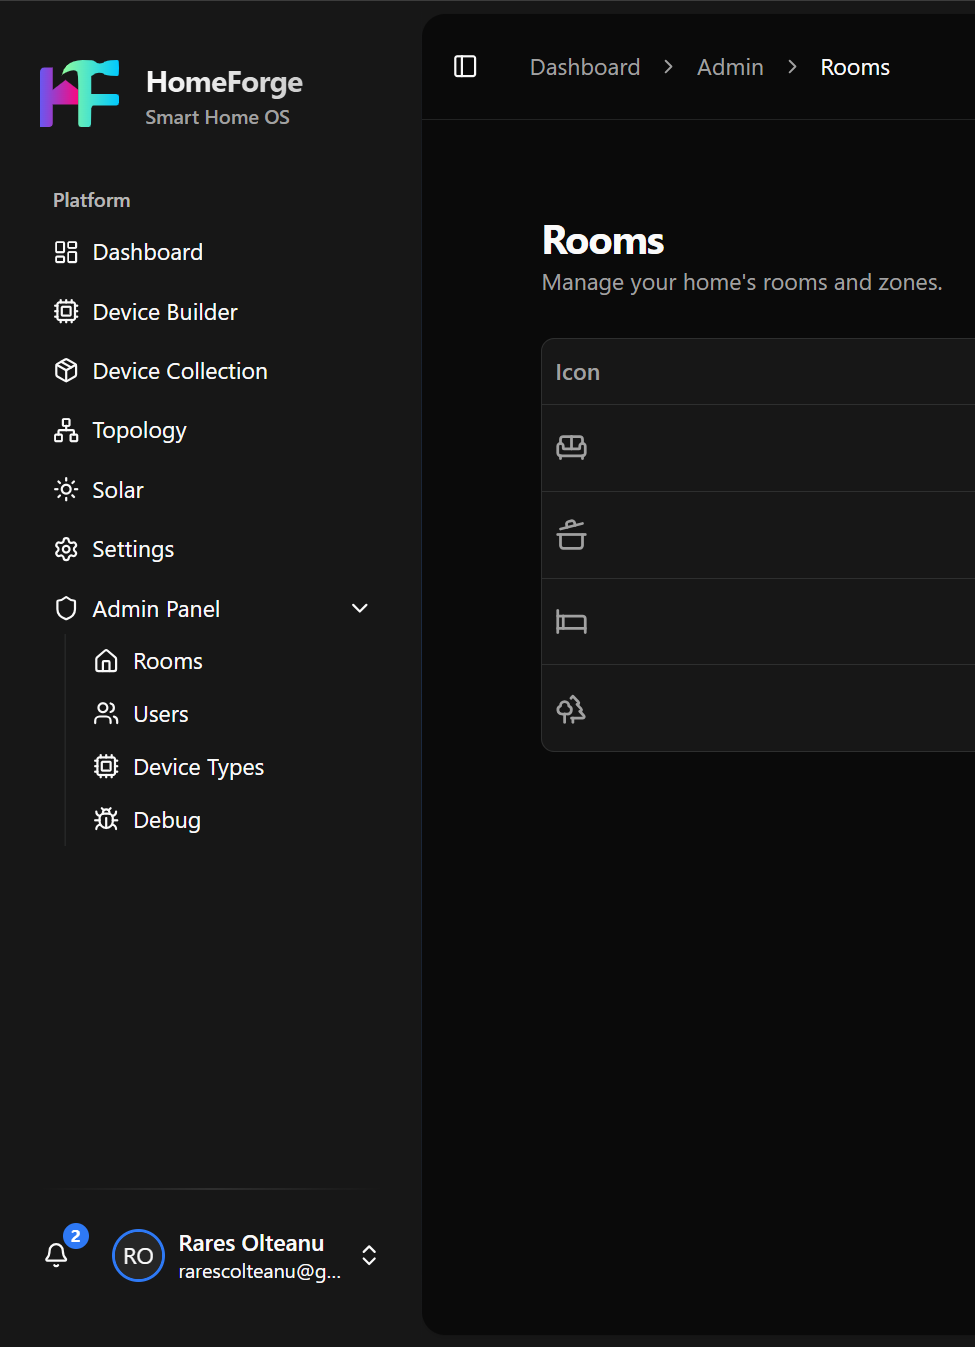
\includegraphics[width=0.5\textwidth]{figuri/sidebar_admin.png}
    \caption{Sidebar-ul HomeForge cu sub-meniul \emph{Admin Panel} activ (screenshot de adăugat)}
    \label{fig:sidebar_admin}
\end{figure}

\subsection{Breadcrumb-uri dinamice}
Componenta \texttt{DynamicBreadcrumbs} citește path-ul curent prin \texttt{usePathname()} din \texttt{next/navigation} și îl segmentează automat. Asta înseamnă că la \texttt{/dashboard/admin/device-types?filter=pending} apar trei breadcrumb-uri (\emph{Dashboard $>$ Admin $>$ Device Types}) fără ca eu să fi configurat ceva explicit. Capitalizarea, hyphen-to-space și link-urile către nivelurile părinte se calculează în timpul randării.

\subsection{Tema și culorile de accent}
Tema light/dark este oferită de pachetul \texttt{next-themes}, care setează un atribut \texttt{class} pe \texttt{<html>}. Butonul \texttt{ModeToggle} din header comută între cele două.

Pe lângă temă, fiecare utilizator își poate alege o \emph{culoare de accent}. Valorile disponibile sunt declarate în \texttt{components/user-provider.tsx}:
\begin{minted}{typescript}
export const ACCENT_COLORS = {
  default: "oklch(0.205 0 0)",
  violet:  "oklch(0.5 0.2 280)",
  blue:    "oklch(0.5 0.2 250)",
  green:   "oklch(0.6 0.15 150)",
  orange:  "oklch(0.6 0.15 50)",
  pink:    "oklch(0.6 0.2 340)",
  cyan:    "oklch(0.6 0.15 200)",
}
\end{minted}
Sunt definite în spațiul de culoare OKLCH (preferabil fa\c{t}\u{a} de RGB pentru consistență perceptivă), iar funcția \texttt{applyAccentColor} setează direct variabilele CSS \texttt{--primary} și \texttt{--ring} pe \texttt{document.documentElement}, fără reload. Preferința este persistată pe server (câmpul \texttt{accent\_color} din \texttt{Profile} — vezi Capitolul 3) și replicată în \texttt{localStorage} pentru a evita „flash"-ul vizual la prima încărcare; un \texttt{useLayoutEffect} aplică culoarea înainte de paint.

% FIGURĂ DE ADĂUGAT: două screenshot-uri ale aceleiași pagini Settings,
% unul cu accent violet și unul cu accent cyan, alăturate, pentru a arăta
% cum se schimbă instantaneu tema.
\begin{figure}[htbp]
    \centering
    % \includegraphics[width=0.95\textwidth]{figuri/accent_colors.png}
    \caption{Aceea\c{s}i pagină \emph{Settings} cu două accent colors diferite (screenshot de adăugat)}
    \label{fig:accent_colors}
\end{figure}

\subsection{\texttt{UserProvider} — sursa unică de adevăr pe client}
\texttt{components/user-provider.tsx} expune un Context React care:
\begin{itemize}
    \item încarcă profilul curent la mount (\texttt{loadUser}) — întâi din \texttt{localStorage} pentru a evita „flash of unauthenticated content", apoi se actualizează cu răspunsul real al lui \texttt{fetchProfile()};
    \item aplică culoarea de accent;
    \item gestionează logout-ul: golește cache-ul TanStack Query (\texttt{queryClient.clear()}), șterge token-urile, șterge layout-ul cache-uit local și redirecționează la \texttt{/login}.
\end{itemize}
Importanța pașilor de cleanup la logout nu este teoretică: fără \texttt{queryClient.clear()}, dacă un alt utilizator se loghează imediat după pe același browser, ar vedea pentru câteva secunde dispozitivele utilizatorului precedent.

\section{Stratul de comunicare cu API-ul}
Toate apelurile către backend sunt concentrate în fișierul \texttt{apiClient.js}, scris în JavaScript pur. Alegerea de a nu folosi TypeScript pentru acest modul a fost deliberată: păstrează codul la nivelul unui apel \texttt{fetch} standard și facilitează parcurgerea sa de către cititori familiarizați cu API-ul \texttt{fetch} al browserelor.

\subsection{Determinarea URL-ului backend-ului}
Frontend-ul nu cunoaște la build-time IP-ul gazdei pe care va rula. Funcția \texttt{getBackendUrl} folosește locația curentă a browserului și înlocuiește portul cu 8000:
\begin{minted}{javascript}
export function getBackendUrl() {
  if (typeof window !== 'undefined') {
    return `${window.location.protocol}//${window.location.hostname}:8000`;
  }
  return 'http://localhost:8000';
}
\end{minted}
Practic, dacă un utilizator accesează aplicația de pe \texttt{http://192.168.1.10:3000}, cererile vor merge automat către \texttt{http://192.168.1.10:8000}, fără configurări suplimentare.

\subsection{Gestiunea token-urilor JWT}
La login, token-ul de acces și cel de refresh sunt stocate în \texttt{localStorage}. Toate cererile autentificate trec prin \texttt{fetchWithAuth}, care:
\begin{enumerate}
    \item adaugă antetul \texttt{Authorization: Bearer <token>};
    \item dacă răspunsul este \texttt{401}, apelează \texttt{refreshAccessToken()} și reîncearcă cererea o singură dată;
    \item dacă reîmprospătarea eșuează, șterge token-urile și aruncă o eroare cu \texttt{status = 401}, care este capturată de \texttt{dashboard/layout.tsx} și care redirecționează către \texttt{/login}.
\end{enumerate}
\begin{minted}{javascript}
async function fetchWithAuth(url, options = {}) {
  const headers = { ...options.headers, ...getAuthHeaders() };
  let res = await fetch(url, { ...options, headers });
  if (res.status === 401) {
    const newToken = await refreshAccessToken();
    const newHeaders = { ...options.headers, Authorization: `Bearer ${newToken}` };
    res = await fetch(url, { ...options, headers: newHeaders });
  }
  return res;
}
\end{minted}

\subsection{Tratarea uniformă a erorilor}
Funcția \texttt{handleApiError} parsează formatul standard al erorilor returnate de Django REST Framework. Aceasta gestionează trei cazuri: un câmp \texttt{detail} (de obicei la erori de permisiune), un câmp \texttt{non\_field\_errors} (la validări la nivel de serializer) și restul, în care fiecare cheie este un câmp specific cu o listă de mesaje. Mesajele sunt concatenate și aruncate ca un singur \texttt{Error}, pe care UI-ul îl afișează prin \texttt{toast.error}.

\section{Gestiunea stării: TanStack Query}
HomeForge folosește \textit{TanStack Query} (denumit anterior React Query) pentru toate datele la nivel de aplicație. \texttt{QueryProvider} este montat în root-ul aplicației (\texttt{components/query-provider.tsx}) și expune un singur \texttt{QueryClient}. Fiecare componentă apoi consumă două hook-uri: \texttt{useQuery} pentru fetch-uri (lista de dispozitive, profilul, notificările) și \texttt{useMutation} pentru scrieri (toggle, update, delete). Două decizii de configurare merită evidențiate: lista de dispozitive folosește \texttt{refetchInterval: 3000} (polling la 3 secunde, înlocuind o eventuală conexiune WebSocket), iar contorul de notificări necitite folosește \texttt{refetchInterval: 30000} (30 de secunde, suficient pentru un badge fără a încărca inutil backend-ul).

\section{Dashboard-ul principal}
Pagina \texttt{app/dashboard/page.tsx} orchestrează trei surse de date — dispozitive, tipuri de dispozitive și camere — și le combină într-un singur grid. Există cinci moduri de grupare expuse într-un \texttt{<Select>}:
\begin{itemize}
    \item \texttt{all} — toate dispozitivele, în ordinea aleasă de utilizator (mod cu drag-and-drop);
    \item \texttt{room} — grupare pe cameră;
    \item \texttt{type} — grupare pe tipul de dispozitiv;
    \item \texttt{status} — grupare pe \texttt{Online} / \texttt{Offline} / \texttt{Error};
    \item \texttt{name} — sortare alfabetică simplă.
\end{itemize}
La nivel de cod, modul curent (\texttt{viewMode}) este oglindit într-o variabilă \texttt{deviceOrder} pe care \texttt{useDashboardLayout} o sincronizează cu serverul prin endpoint-ul \texttt{PATCH /api/device-order/}. Preferința utilizatorului supraviețuiește între dispozitive.

\subsection{Hook-ul \texttt{useDashboardLayout}}
Logica de layout este izolată într-un singur hook (\texttt{hooks/useDashboardLayout.ts}). Acesta:
\begin{enumerate}
    \item descarcă layout-ul curent prin \texttt{useQuery(['dashboardLayout'], fetchDashboardLayout)} cu \texttt{staleTime: Infinity};
    \item dacă API-ul eșuează (mod offline), cade pe \texttt{localStorage} ca rezervă;
    \item \textit{reconciliază} layout-ul cu lista actuală de dispozitive — elimină referințele către cele șterse, adaugă cele noi, dizolvă folderele rămase cu mai puțin de 2 elemente (vezi \texttt{reconcileLayout} în \texttt{lib/dashboard-grid.ts});
    \item expune funcții de mutație: \texttt{moveItem}, \texttt{createFolder}, \texttt{addToFolder}, \texttt{removeFromFolder}, \texttt{renameFolder}, \texttt{dissolveFolder}, \texttt{resetLayout}, \texttt{revertToShared};
    \item salvează modificările pe server cu \texttt{debounce} de 800 ms și \textit{flush} imediat la ieșirea din modul de editare („Done”).
\end{enumerate}

\begin{minted}{typescript}
const scheduleSave = useCallback((newLayout: DashboardLayout) => {
  saveLayout(newLayout);                         // localStorage instantaneu
  if (saveTimerRef.current) clearTimeout(saveTimerRef.current);
  hasPendingSaveRef.current = true;
  saveTimerRef.current = setTimeout(() => {
    saveToApi(newLayout);                        // API după 800 ms
  }, 800);
}, [saveToApi]);
\end{minted}

\subsection{Drag-and-drop și foldere}
Componenta \texttt{DraggableDeviceGrid} folosește biblioteca \texttt{@dnd-kit/core} pentru drag-and-drop. Fiecare card este învelit într-un \texttt{SortableGridItem} cu trei zone de drop:
\begin{itemize}
    \item zona \emph{stângă}: dispozitivul tras este inserat înaintea țintei;
    \item zona \emph{dreaptă}: este inserat după;
    \item zona \emph{mijloc}: dispozitivele se combină într-un folder nou (sau dispozitivul este adăugat în folderul țintă).
\end{itemize}
Constrângerile semantice (un folder are între 2 și 4 dispozitive, fiecare \texttt{deviceId} apare cel mult o dată) sunt verificate atât pe client cât și pe backend (vezi \texttt{DashboardLayoutSerializer} în Capitolul 3).

% FIGURĂ DE ADĂUGAT: screenshot al dashboard-ului în mod „edit” — se văd cardurile,
% un folder deschis cu 3 dispozitive, plus indicatorii de drop (stânga / mijloc / dreapta).
\begin{figure}[htbp]
    \centering
    % \includegraphics[width=0.95\textwidth]{figuri/dashboard_edit_mode.png}
    \caption{Dashboard-ul HomeForge în modul de editare a layout-ului (screenshot de adăugat)}
    \label{fig:dashboard_edit}
\end{figure}

\section{Cardurile inteligente: \texttt{SmartDeviceCard}}
Componenta \texttt{SmartDeviceCard} este probabil cea mai densă din întregul frontend, fiindcă rezolvă în același loc trei probleme dificile: randarea dinamică a unui număr variabil de widget-uri, optimistic UI și combaterea \textit{glitch}-urilor de stare la apăsări rapide.

\subsection{Randarea condusă de \texttt{card\_template}}
Fiecare tip de dispozitiv definește o listă de \texttt{controls}, în care fiecare element are un \texttt{widget\_type}. Componenta apelează funcția internă \texttt{renderWidget(control, index)}, care selectează implementarea vizuală corespunzătoare: \texttt{Switch} pentru \texttt{TOGGLE}, \texttt{Slider} pentru \texttt{SLIDER} sau widget-uri specializate definite în \texttt{SensorWidgets.tsx} (\texttt{TemperatureWidget}, \texttt{HumidityWidget} etc.). Fiecare widget primește valoarea curentă prin câmpul \texttt{variable\_mapping}, mecanism care permite aceleiași componente să servească orice tip de dispozitiv definit prin device builder.

Layout-ul cardului are două variante: \emph{row} (widget-uri pe linie, util pentru dispozitive simple) și \emph{square} (widget-uri pătrate, util pentru senzori). Layout-ul de grid se citește dintr-un câmp \texttt{layout\_config} cu chei \texttt{w} (numărul de coloane) și \texttt{gap}; componenta convertește \texttt{layout\_config.w} sau \texttt{layout\_config.columns} în clase Tailwind (\texttt{grid-cols-1/2/3}).

Există și un caz special: \texttt{isSingleToggleDevice(controls)}. Dacă un dispozitiv are exact un singur control de tip \texttt{TOGGLE} și nimic altceva (un releu pentru un bec, de exemplu), cardul devine \emph{tap-to-toggle} — întreaga suprafață a cardului acționează ca un switch, fără un widget separat. Detaliul îmbunătățește vizibil ergonomia pe mobil.

\subsection{Pattern-ul \textit{Optimistic UI}}
Această subsecțiune descrie mecanismul central de gestiune a stării interactive. La apăsarea unui toggle, componenta:
\begin{enumerate}
    \item construiește noua stare locală \texttt{newState = \{...currentState, [variable]: value\}};
    \item o salvează imediat în \texttt{useState}, deci UI-ul se actualizează în 0 milisecunde;
    \item programează un \texttt{setTimeout} de 50 ms (pentru toggle, ca să consolideze apăsările repetate) sau 500 ms (pentru slider, ca să nu trimită zeci de cereri per gest) — un \textit{debounce} clasic;
    \item după timer, declanșează mutația TanStack Query, care apelează \texttt{updateDeviceState(id, newState)}.
\end{enumerate}

Mutația utilizează patru dintre hook-urile expuse de \texttt{useMutation} — \texttt{mutationFn}, \texttt{onMutate}, \texttt{onError} și \texttt{onSettled}. Hook-ul \texttt{onSuccess} este omis deliberat, din motive explicate mai jos. Scheletul implementării, în formă condensată:
\begin{minted}{typescript}
const updateMutation = useMutation({
  mutationFn: ({ id, newState }) => updateDeviceState(id, newState),
  onMutate: async ({ id, newState }) => {
    await queryClient.cancelQueries({ queryKey: ['devices'] });
    const previousDevice = queryClient.getQueryData(['device', id]);
    queryClient.setQueryData(['device', id], (old) => ({ ...old, current_state: newState }));
    return { previousDevice };                       // pasat la onError pentru rollback
  },
  onError:   (_e, _v, ctx) => { /* rollback la ctx.previousDevice + toast.error */ },
  onSettled: () => { /* setIsRefetching(true); invalidate cu delay; timeout siguranță 5s */ },
});
\end{minted}

Câteva detalii subtile pe care le-am implementat după mai multe iterații:
\begin{itemize}
    \item \texttt{onMutate} salvează starea anterioară într-un \textit{context} care, în caz de eroare, este folosit pentru \emph{rollback}. Fără aceasta, dacă dispozitivul este offline, butonul ar rămâne blocat în starea optimistă incorectă.
    \item Intenționat \emph{nu} folosesc \texttt{onSuccess} pentru a suprascrie starea locală: serverul răspunde imediat cu \texttt{HTTP 202} și o stare anticipată, dar starea reală vine asincron, de pe MQTT. Dacă aș suprascrie pe \texttt{onSuccess}, butonul ar putea „sări” înapoi câteva secunde mai târziu.
    \item \texttt{onSettled} marchează \texttt{isRefetching = true}, ceea ce face ca UI-ul să afișeze un \texttt{Loader2} suprapus. Există un timeout de siguranță (5 secunde) care anulează această stare dacă backend-ul nu mai răspunde — nu vrem ca utilizatorul să rămână blocat cu un \textit{spinner} infinit.
    \item Există un \texttt{useEffect} care detectează când starea de pe server „a ajuns din urmă” starea optimistă (toate cheile modificate sunt egale) și, în acel moment, oprește \texttt{isRefetching}, iar vizual butonul rămâne în stare „sincronizare” doar atât timp cât chiar este o discrepanță reală între ce vrem și ce raportează firmware-ul.
\end{itemize}

% FIGURĂ DE ADĂUGAT: diagrama temporală a unei apăsări — buton apăsat la t=0,
% UI optimist la t=0+ε, debounce până la t=50ms, request HTTP, răspuns 202 la t=100ms,
% publicare MQTT, ESP32 toggle releu la t=180ms, publish state, listener Django,
% refresh listă dispozitive la t=300ms, sincronizat la t=350ms. Poate fi
% o diagramă de tip swim-lane în draw.io.
\begin{figure}[htbp]
    \centering
    % 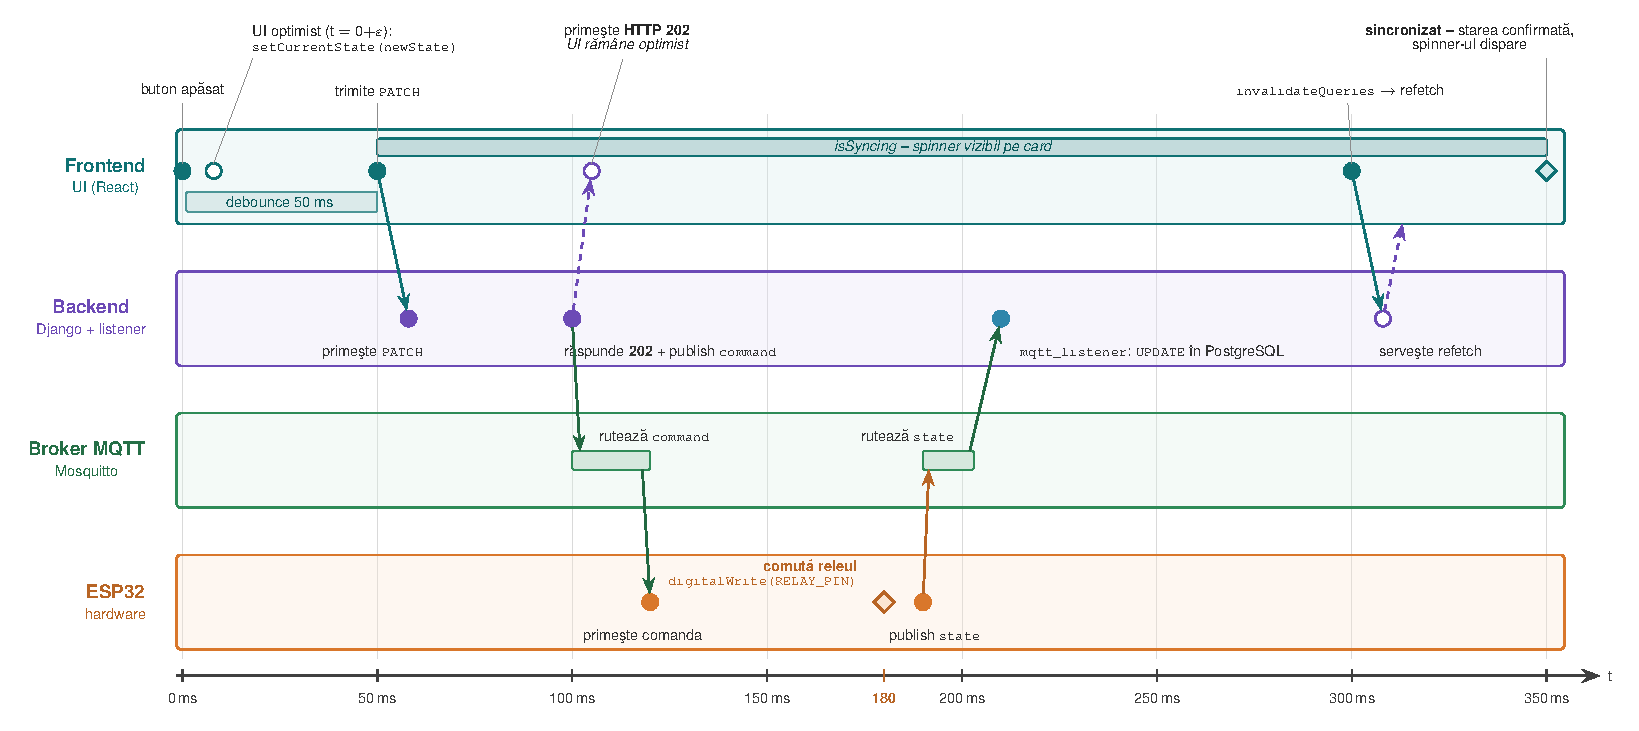
\includegraphics[width=0.95\textwidth]{figuri/optimistic_ui_timeline.pdf}
    \caption{Diagrama temporală a unei apăsări de toggle în interfața HomeForge (figură de adăugat)}
    \label{fig:optimistic_timeline}
\end{figure}

\section{Centrul de notificări}
\texttt{notification-center.tsx} este componenta din colțul dreapta-sus al headerului. Este un \texttt{Popover} care afișează lista alertelor curente:
\begin{itemize}
    \item folosește două \texttt{useQuery} — unul pentru lista completă, unul pentru contorul de necitite, ambele cu \texttt{refetchInterval: 30000};
    \item iconițele și culorile sunt alese în funcție de \texttt{notification\_type} (\texttt{device\_offline}, \texttt{device\_type\_pending}, etc.);
    \item \texttt{action\_url}-ul venit de la backend este normalizat printr-o funcție \texttt{getActionUrl} care adaugă prefixul \texttt{/dashboard} și redirecționează URL-urile către individuale (\texttt{/admin/device-types/22}) către pagina-listă cu filtru (\texttt{/dashboard/admin/device-types?filter=pending}).
\end{itemize}

\section{Vizualizarea topologiei}
Pagina \texttt{/dashboard/topology/} se bazează pe biblioteca \texttt{@xyflow/react} (React Flow v12). Datele vin direct de la endpoint-ul \texttt{GET /api/topology/}, în formatul cerut nativ de React Flow (\texttt{nodes[]} și \texttt{edges[]}). Logica frontend este în \texttt{TopologyCanvas.tsx} și are două componente:

\begin{enumerate}
    \item Un algoritm propriu de layout ierarhic care plasează gateway-ul în stânga și dispozitivele într-o coloană verticală în dreapta, cu \texttt{childXOffset = 450} și \texttt{childSpacingY = 180} pixeli. Renunțarea la un algoritm generic precum ELK sau Dagre este motivată de profilul tipic al rețelei vizualizate: pentru un număr de dispozitive cuprins între 5 și 30, o dispunere în coloană oferă cea mai bună lizibilitate.
    \item Un mecanism de păstrare a selecției: utilizatorul poate selecta unul sau mai multe noduri, iar la re-randarea automată (lista de dispozitive se actualizează la fiecare 3 secunde), un \texttt{useRef} numit \texttt{selectionRef} reține ce a fost selectat și restaurează starea pe noile noduri.
\end{enumerate}

Nodurile sunt randate de patru componente custom în \texttt{topology/nodes/}: \texttt{BuilderStyleNode}, \texttt{GlassDeviceNode}, \texttt{TopologyBuilderNode}, \texttt{UnifiDeviceNode}. \texttt{TopologyBuilderNode} este cea folosită în mod implicit; celelalte sunt variante stilistice între care utilizatorul poate alege.

\section{Editorul vizual de tipuri de dispozitive (\textit{device builder})}
Una dintre cele mai interesante pagini este \texttt{device-builder/DeviceUICreator.tsx}, un editor vizual cu două panouri:
\begin{itemize}
    \item în stânga, un \emph{node graph} (bazat tot pe React Flow) unde utilizatorul adaugă microcontrolere și senzori, conectându-i între ei. Fiecare nod are un ID unic care va fi referențiat din widget-urile vizuale;
    \item în dreapta, lista \emph{widget-urilor} (toggle, slider, sensor) care vor compune cardul dispozitivului. Fiecare widget este legat de un nod prin câmpul \texttt{variable\_mapping}.
\end{itemize}

În jurul editorului există trei panouri auxiliare:
\begin{itemize}
    \item \texttt{FirmwareCodeEditor.tsx} — editor de cod Arduino bazat pe \texttt{prismjs} și \texttt{react-simple-code-editor};
    \item \texttt{WiringDiagramEditor.tsx} — încărcare de schemă electrică (imagine) și descriere textuală;
    \item \texttt{DocumentationEditor.tsx} — editor Markdown cu randare \texttt{react-markdown} (cu \texttt{remark-gfm} și \texttt{rehype-highlight}).
\end{itemize}

La finalul fluxului, utilizatorul apasă \emph{Propose} și aplicația apelează \texttt{POST /api/device-types/propose/} cu o structură JSON compusă din:
\begin{itemize}
    \item \texttt{name} — denumirea tipului;
    \item \texttt{definition.structure[]} — noduri și conexiuni (microcontroler, senzori, pini, fire);
    \item \texttt{card\_template.controls[]} — widget-urile vizuale;
    \item \texttt{firmware\_code}, \texttt{wiring\_diagram\_text}, \texttt{documentation} — text;
    \item \texttt{wiring\_diagram\_base64}, \texttt{documentation\_images\_base64} — imagini encodate.
\end{itemize}
Validatorul de backend (\texttt{CustomDeviceTypeSerializer.validate}) verifică explicit că fiecare \texttt{variable\_mapping} din widget-uri corespunde unui ID definit în \texttt{structure[]} — astfel, este imposibil să propui un tip de dispozitiv „rupt”.

% FIGURĂ DE ADĂUGAT: screenshot al device builder-ului — în stânga node-graph
% cu un ESP32 conectat la DHT11 și un releu, în dreapta lista de widget-uri (un
% TOGGLE pentru releu, un TEMPERATURE pentru DHT11, un HUMIDITY pentru DHT11).
\begin{figure}[htbp]
    \centering
    % 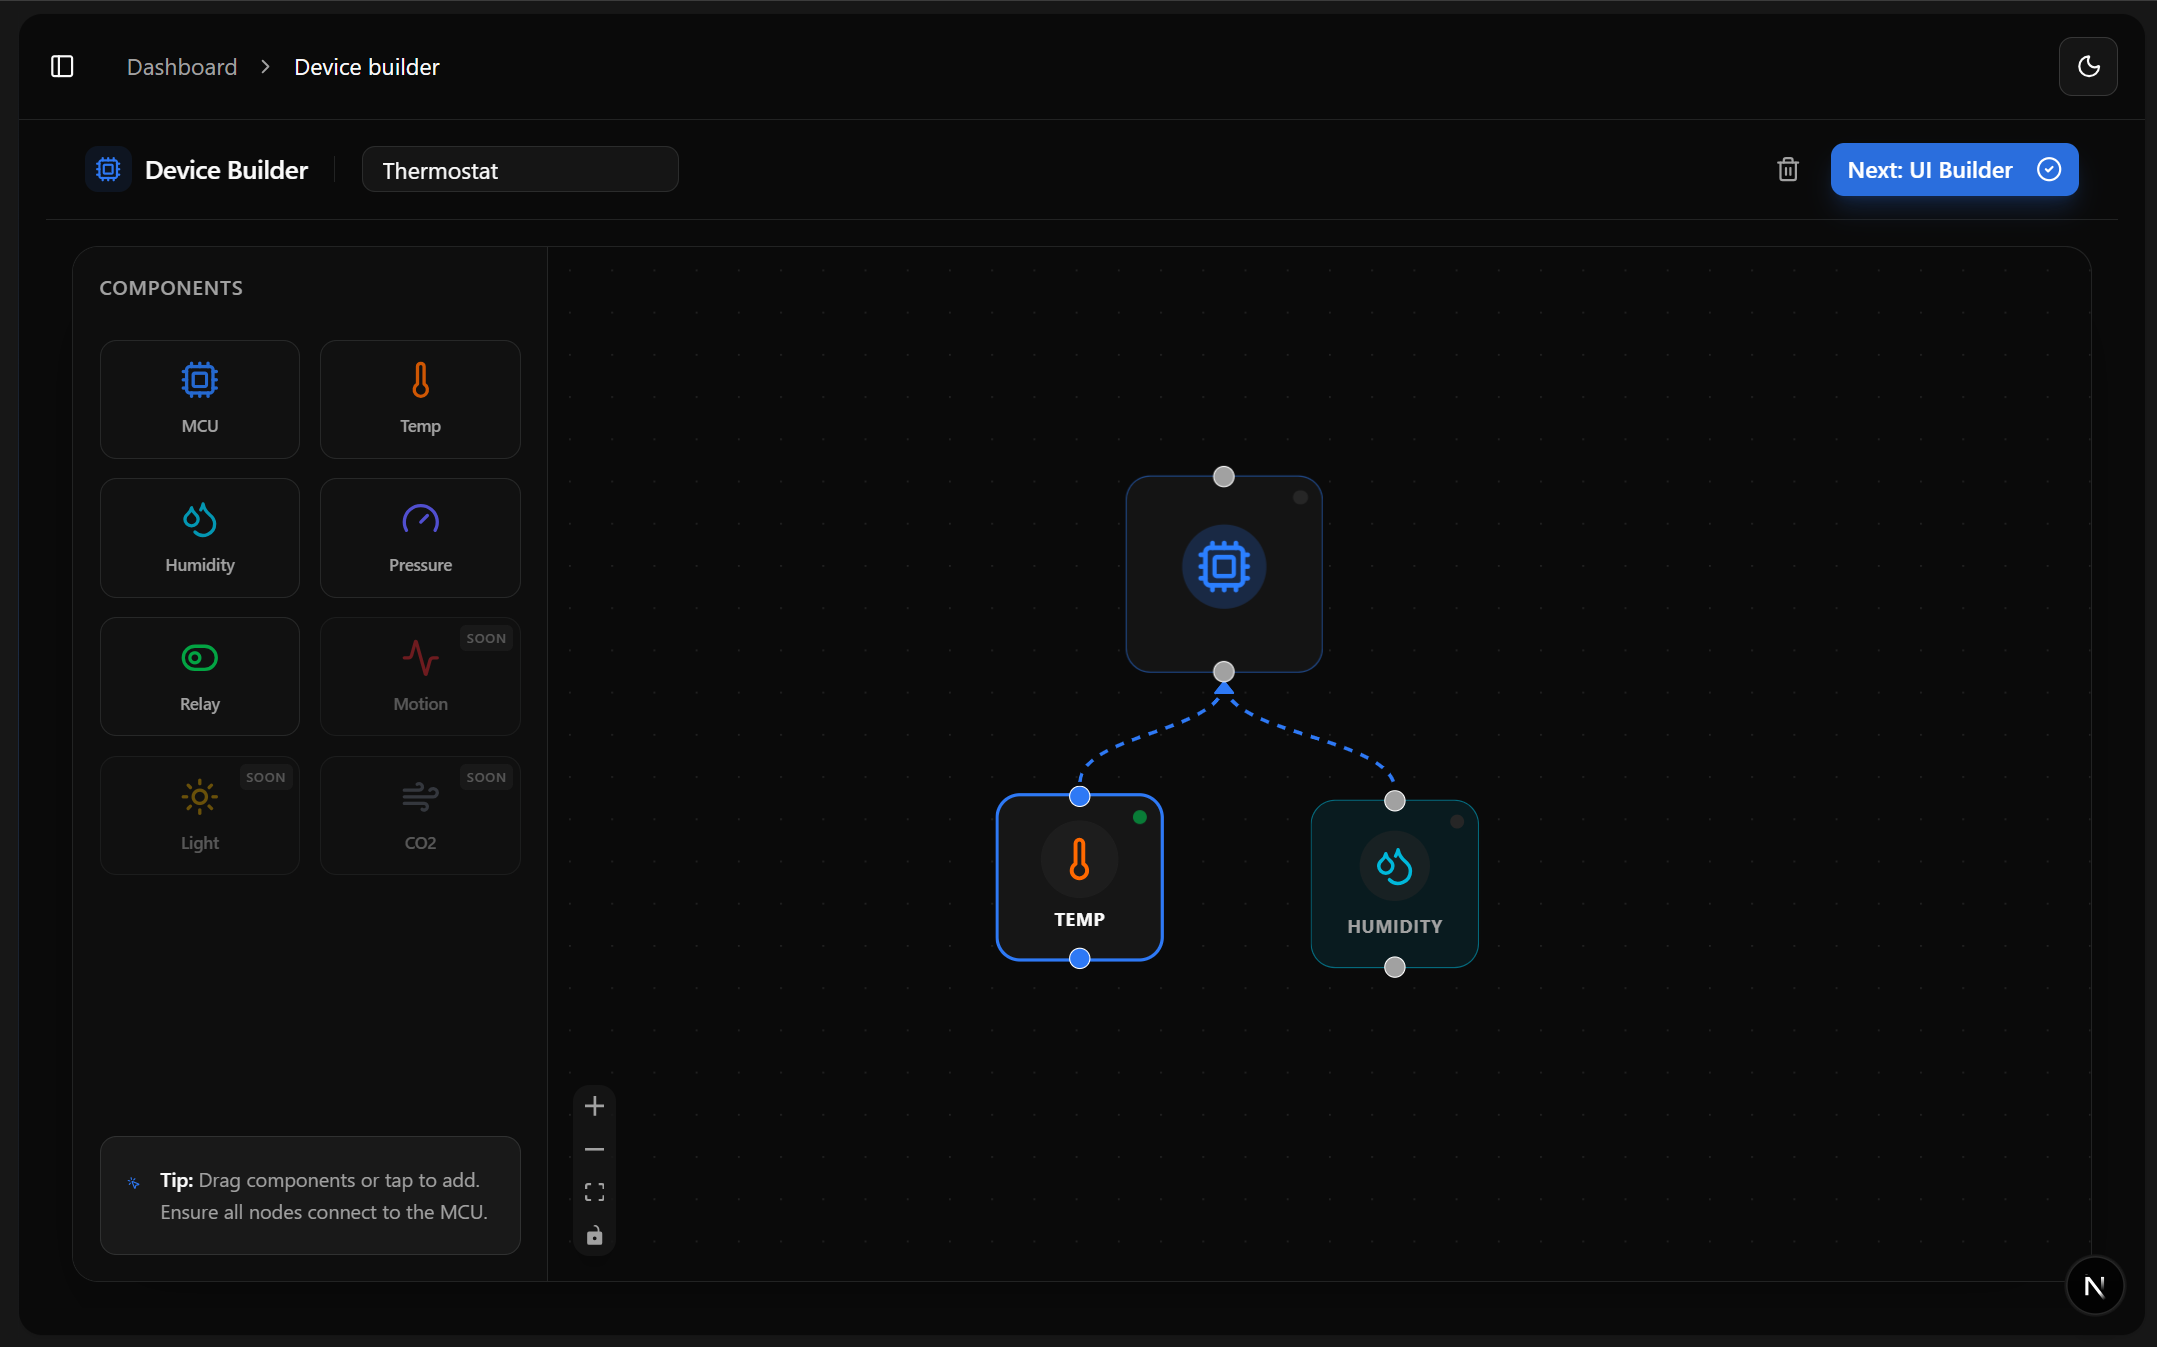
\includegraphics[width=0.95\textwidth]{figuri/device_builder.png}
    \caption{Device builder-ul HomeForge cu un node graph și panoul de widget-uri (screenshot de adăugat)}
    \label{fig:device_builder}
\end{figure}

\section{Setup wizard-ul}
La primul vizit pe o instanță proaspătă, \texttt{SetupWizard.tsx} ghidează utilizatorul printr-un flux în 5 pași: \emph{welcome} → \emph{account} → \emph{rooms} → \emph{devices} → \emph{complete}. Pașii sunt componente separate în \texttt{components/setup/steps/} și comunică prin \texttt{onNext} / \texttt{onBack} cu containerul. La pasul \emph{account}, contul creat devine automat \texttt{owner}, fiindcă serverul răspunde la \texttt{POST /register/} cu \texttt{is\_first\_user} activat (vezi Capitolul 3). La pasul \emph{devices}, utilizatorul poate importa tipurile predefinite prin endpoint-ul \texttt{POST /api/device-types/import-defaults/}.

Indicatorul de progres este o linie întreruptă în patru segmente; fiecare segment primește clase Tailwind diferite pe baza indexului pasului curent. Animațiile de tranziție folosesc \texttt{animate-in fade-in duration-300} — o clasă utilitară oferită de pluginul \texttt{tw-animate-css}.

\section{Onboarding-ul: \texttt{OnboardingChecklist} și \texttt{PageTooltip}}
Asistentul de configurare inițial (\emph{setup wizard}) acoperă doar primii pași de instalare. Pentru utilizatorii care accesează aplicația ulterior, este oferit un mecanism de onboarding suplimentar, mai puțin intruziv, format din două componente complementare situate în \texttt{components/onboarding/}.

\paragraph{Checklist-ul de pe dashboard.} Componenta \texttt{OnboardingChecklist.tsx} este un card afișat în partea superioară a dashboard-ului, vizibil până la finalizarea tuturor pașilor recomandați: crearea contului, definirea a cel puțin unei camere, importul a cel puțin unui tip de dispozitiv și adăugarea primului dispozitiv. Verificarea condițiilor utilizează contoarele primite prin \texttt{props}, cu fallback către apelurile \texttt{fetchRooms()}, \texttt{fetchDeviceTypes()} și \texttt{fetchDevices()}; pașii satisfăcuți sunt marcați automat ca \emph{completați}. Pașii suplimentari sunt persistați în \texttt{localStorage} sub cheia \texttt{onboarding\_checklist\_completed}, iar butonul \emph{Dismiss} setează flag-ul \texttt{onboarding\_checklist\_dismissed = true}.

\paragraph{Tooltip-urile de pagină.} Componenta \texttt{PageTooltip.tsx} este reutilizabilă și se inserează o singură dată pe fiecare pagină principală. Vizibilitatea este controlată prin \texttt{localStorage} (cheia \texttt{visited\_pages}): tooltip-ul se afișează exclusiv la prima vizită, cu dispariție automată după 8,5 secunde sau prin acțiune explicită a utilizatorului (buton de închidere). Mesajele sunt specifice fiecărei pagini — pe dashboard, de exemplu, textul afișat este: \emph{„This is your control center. Add devices, organize them into rooms, and monitor everything in real time."}

% FIGURĂ DE ADĂUGAT (combinată, 4 panel-uri 2×2): (sus-stânga) setup wizard
% pasul „account", (sus-dreapta) setup wizard pasul „devices" cu lista
% predefinite, (jos-stânga) dashboard cu OnboardingChecklist activ,
% (jos-dreapta) un PageTooltip deschis pe o pagină interioară.
\begin{figure}[htbp]
    \centering
    % \includegraphics[width=0.95\textwidth]{figuri/onboarding_combo.png}
    \caption{Fluxul complet de onboarding: setup wizard (sus) și mecanismele de onboarding ulterior (jos) (screenshot de adăugat)}
    \label{fig:onboarding_combo}
\end{figure}

\section{Pagina de setări}
\texttt{app/dashboard/settings/page.tsx} grupează într-un singur formular controlat patru zone funcționale: profilul de bază (nume, email, username, parolă nouă cu confirmare), avatarul (\texttt{FileReader} pentru preview, \texttt{FormData} la salvare; backend-ul generează un nume UUID și șterge prin semnal \texttt{pre\_save} avatarul vechi), paleta de \emph{accent colors} (cele 7 valori OKLCH din \texttt{ACCENT\_COLORS}, aplicate instant prin \texttt{updateAccentColor}) și un panou read-only cu rolul curent și informații despre cont. Salvarea apelează \texttt{updateProfile} din \texttt{apiClient.js} (un \texttt{PUT /api/me/} multipart), iar la succes invocă \texttt{refreshUser()} ca să-și reîmprospăteze starea contextului de utilizator — fără asta, o schimbare de nume nu s-ar reflecta imediat în sidebar.

% FIGURĂ DE ADĂUGAT: screenshot al paginii Settings — partea de sus cu profil
% și avatar, partea de jos cu paleta de 7 cercuri pentru accent color. Sugestie:
% poți face screenshot cu o culoare violet/cyan selectată pentru a se vedea.
\begin{figure}[htbp]
    \centering
    % \includegraphics[width=0.85\textwidth]{figuri/settings_page.png}
    \caption{Pagina de setări a utilizatorului, cu paleta de \emph{accent colors} (screenshot de adăugat)}
    \label{fig:settings_page}
\end{figure}

\section{Adăugarea unui dispozitiv: \texttt{AddDeviceDialog}}
Adăugarea unui dispozitiv reprezintă una dintre cele mai frecvente acțiuni efectuate de utilizator, motiv pentru care a fost implementată sub forma unui dialog multi-pas: \texttt{AddDeviceDialog.tsx}. Componenta este un \texttt{Dialog} construit din primitive shadcn/ui peste Radix, cu trei pași: (1) selectarea tipului de dispozitiv dintr-o listă filtrată după \texttt{approved=true}, (2) completarea formularului cu nume, adresă IP (validată local), cameră (prin \texttt{Select}) și o iconiță aleasă prin componenta \texttt{IconPicker}, (3) ecranul de confirmare și transmiterea cererii \texttt{registerDevice}. Datele necesare sunt încărcate printr-un singur apel \texttt{Promise.all([fetchDeviceTypes(), fetchRooms()])} la deschidere; după înregistrarea cu succes, \texttt{onDeviceAdded} declanșează un \texttt{window.location.reload()} — soluție simplă, care poate fi înlocuită în versiuni ulterioare cu \texttt{queryClient.invalidateQueries}. Componenta \texttt{IconPicker} este un \texttt{Popover} care expune întregul set de iconițe Lucide (peste 1500 de simboluri) împreună cu un câmp de căutare; filtrarea se face local prin \texttt{useMemo}, limitată la primele 200 de rezultate pentru a păstra timpul de randare scăzut.

% FIGURĂ DE ADĂUGAT: screenshot al AddDeviceDialog la pasul 2, cu formularul
% completat (Nume: „Bec living", IP: „192.168.1.42", Cameră: „Living Room",
% iconița aleasă). Sugestie: poți face câte un screenshot pentru fiecare pas.
\begin{figure}[htbp]
    \centering
    % \includegraphics[width=0.7\textwidth]{figuri/add_device_dialog.png}
    \caption{Dialogul de adăugare a unui dispozitiv nou — pasul de detalii (screenshot de adăugat)}
    \label{fig:add_device_dialog}
\end{figure}

\section{Panoul de administrare}
Pentru utilizatorii cu rol \texttt{admin} sau \texttt{owner}, secțiunea \texttt{/dashboard/admin/} expune cinci pagini de management. Toate verifică încă o dată rolul (\texttt{useUser()} + role check) și au protecții suplimentare la nivel de UI (butoanele destructive sunt mereu confirmate printr-un \texttt{AlertDialog}).

\subsection{Hub-ul: \texttt{/dashboard/admin/}}
Pagina-hub (\texttt{app/dashboard/admin/page.tsx}) este o grilă de patru carduri, fiecare ducând la o sub-secțiune. Sub grila de module există un mic card „System Status" cu două indicatoare verzi pentru \emph{API Services} și \emph{Database Connected} — momentan statice, dar gândite să fie populate într-o iterație viitoare de o cerere către \texttt{GET /api/system-status/}.

\subsection{Aprobarea tipurilor de dispozitive: \texttt{approvals/}}
\texttt{app/dashboard/admin/approvals/page.tsx} reproduce vizualizarea de tip device builder \emph{în interiorul} interfeței de aprobare: două tab-uri (\emph{Pending} și \emph{Denied}), iar pentru fiecare propunere — un mini-grafic React Flow care arată topologia electrică, un preview al cardului UI rezultat (un \texttt{SmartDeviceCard} read-only) și butoanele \emph{Approve} / \emph{Deny} (acesta din urmă obligă completarea unui motiv prin \texttt{Textarea}, validat și pe server). La aprobare, \texttt{useMutation} apelează \texttt{approveDeviceType(id)}, invalidează cache-ul, iar utilizatorul propunător primește automat notificarea „Device Type Approved" (fluxul este declanșat din backend, vezi Capitolul 3).

% FIGURĂ DE ADĂUGAT: screenshot al paginii de Approvals — un tip pending
% afișat cu graful de senzori în stânga și cardul preview în dreapta, plus
% butoanele Approve/Deny.
\begin{figure}[htbp]
    \centering
    % 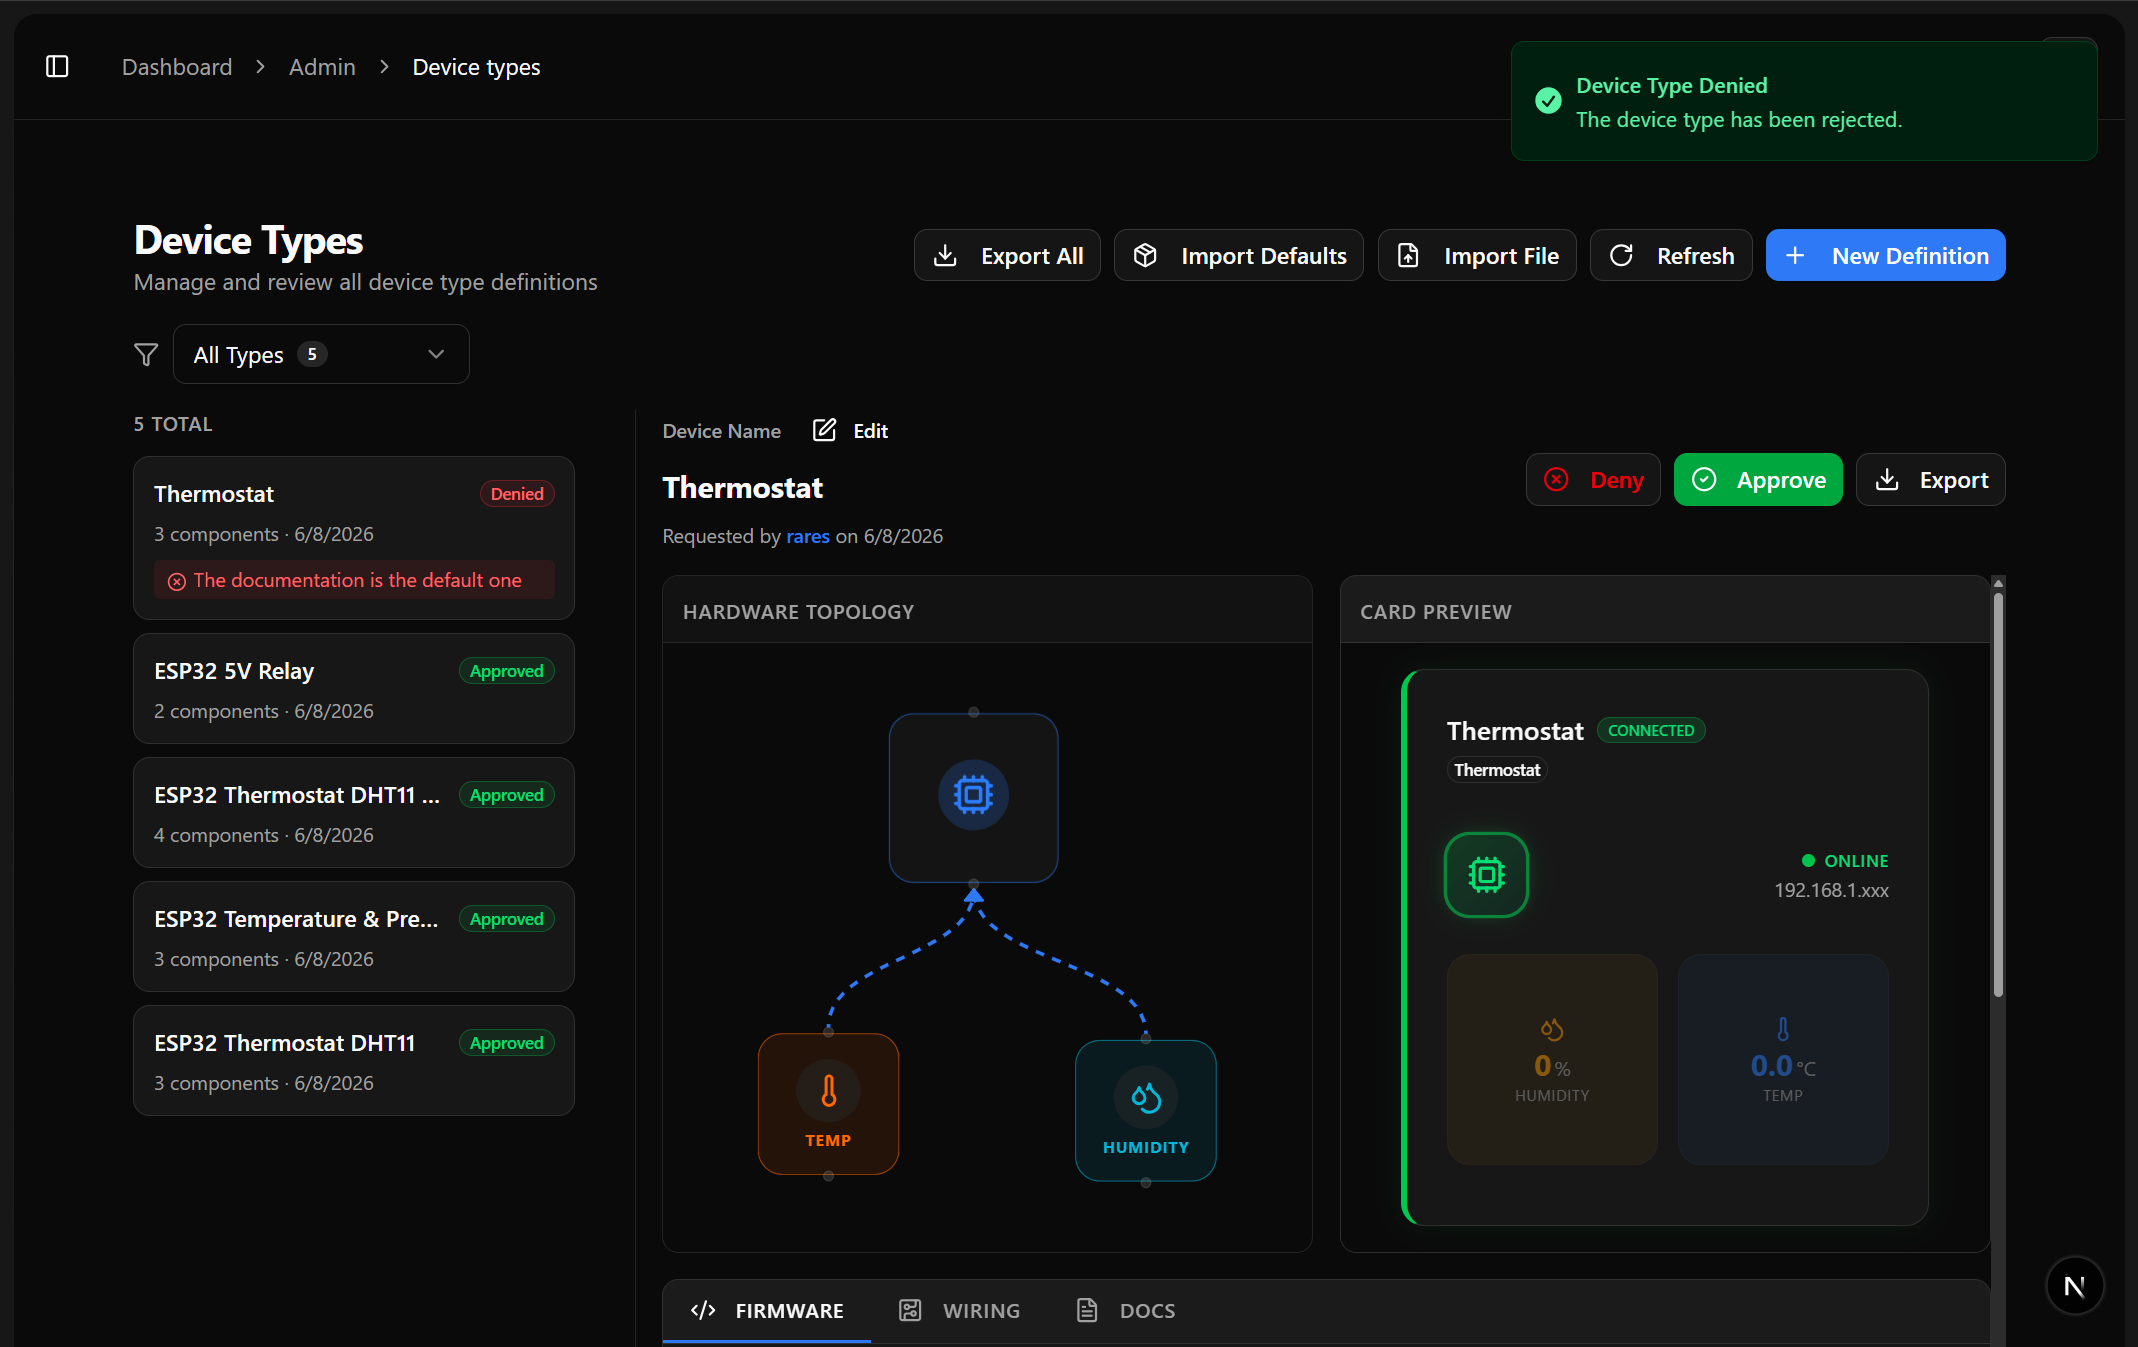
\includegraphics[width=0.95\textwidth]{figuri/admin_approvals.png}
    \caption{Pagina de aprobare a tipurilor de dispozitive propuse de utilizatori (screenshot de adăugat)}
    \label{fig:admin_approvals}
\end{figure}

\subsection{Gestiunea utilizatorilor: \texttt{users/}}
\texttt{app/dashboard/admin/users/page.tsx} afișează un tabel \texttt{Table} (shadcn/ui) cu toți utilizatorii din sistem. Coloanele includ avatar, username, email, rol și un meniu de acțiuni (\texttt{DropdownMenu} cu \texttt{DropdownMenuSub} pentru schimbarea rolului). Filtrul de top oferă o căutare textuală live (controlată local) și un select pentru filtrare după rol. Url-ul acceptă un \texttt{?highlight=<id>} care evidențiază temporar un user — folosit din notificări pentru deep-linking.

\subsection{Camerele, tipurile de dispozitive, debug-ul}
Restul sub-paginilor au design similar. Pe scurt: \texttt{admin/rooms/} face CRUD pe camere folosind \texttt{IconPicker} pentru iconițe (ștergerea unei camere lasă dispozitivele în starea „neasignată" prin \texttt{on\_delete=SET\_NULL}); \texttt{admin/device-types/} listează toate tipurile cu suport pentru import/export JSON și ștergere în bulk a celor respinse; \texttt{admin/debug/} este o pagină de \emph{debugging} unde administratorul poate suprascrie manual starea unui dispozitiv (\texttt{Textarea} cu JSON validat live), forța statusul \texttt{online}/\texttt{offline}/\texttt{error} și trimite comenzi de probă — utilă pentru dezvoltarea UI-ului fără hardware la îndemână.

\section{Recapitulare}
Frontend-ul HomeForge este un Next.js obișnuit, în care complexitatea reală se concentrează în câteva fișiere bine delimitate:
\begin{itemize}
    \item \texttt{apiClient.js} — comunicarea cu API-ul, gestionarea JWT;
    \item \texttt{SmartDeviceCard.tsx} — randarea dinamică a cardurilor și optimistic UI;
    \item \texttt{useDashboardLayout.ts} — layout-ul persistent al dashboard-ului;
    \item \texttt{DeviceUICreator.tsx} — device builder-ul cu graf vizual.
\end{itemize}
Restul codului — sidebar, breadcrumbs, mode toggle, pagini de admin — este aproape integral declarativ, ceea ce reflectă filozofia generală a proiectului: simplitate vizibilă, transparență a fluxului de date.
